%!TEX root = ../tcc.tex

\chapter{Conceitos de Computação no BitTorrent}

O BitTorrent é um protocolo cuja existência depende de vários componentes das mais
variadas áreas de estudo da Computação. Neste capítulo, mostraremos alguns desses
componentes e de que forma o Transmission os implementa, a fim de conseguir desempenhar
bem sua função de cliente BitTorrent.

%!TEX root = ../../tcc.tex

\section{Estruturas de dados}

Conjuntos são tão fundamentais na Ciência da Computação quando na matemática. Os
conjuntos manipulados por algoritmos são, em geral, alterados ao longo do tempo, sendo
chamados de dinâmicos. Alguns algoritmos utilizam conjuntos, realizando diversas
operações sobre eles, como inserção, remoção e testes de pertinência de elementos.
Conjuntos dinâmicos que permitem essas operações são chamados de dicionários
\cite{book:clrs}.

Na linguagem C, geralmente são implementados usando estruturas (\emph{structs}), que são
coleções de variáveis (membros), independentes de tipo, agrupadas sobre o mesmo nome.
Com isso, várias implementações de dicionário foram criadas, cada uma com suas
peculiaridades. Dentre as estruturas utilizadas no Transmission encontramos:

\begin{itemize}
    \item vetores (\emph{arrays});
    \item listas ligadas (\emph{linked lists});
    \item filas (\emph{queues}); e
    \item \glspl*{hashtable} (\emph{hash tables}).
\end{itemize}

%!TEX root = ../../tcc.tex

\subsection*{Vetores}

Vetores (ou \emph{arrays}) são a implementação de vetores matemáticos de maneira
virtual. Na prática, consistem de sequência ou listas de variáveis do mesmo tipo. Na
linguagem C, podem ser declaradas de forma estática ou dinâmica.

Vetores estáticos têm tamanho fixo estabelecido na sua declaração em tempo de
compilação, tendo espaços de memória reservados na pilha de execução de acordo com o
tipo, não podendo ser alterado durante a execução do programa.

\begin{ccode}
    char announce[1024]; // URL de announce
\end{ccode}

Já os vetores dinâmicos são blocos de memória alocados e liberados durante a execução do
programa. Para isso, são utilizados ponteiros para um objeto do mesmo tipo de cada
elemento do vetor. Dessa forma, a memória é reservada em tempo de execução na memória
heap. Assim, pode ter seu tamanho redimensionado conforme a necessidade.

\begin{ccode}
    int *a = malloc( 3*sizeof(int) ); // aloca memoria para um vetor de 3 inteiros
    free(a);                          // desaloca a memoria alocada
\end{ccode}

Apesar dessa diferença, ambos os tipos de vetores funcionam da mesma maneira, usufruindo
da aritmética de ponteiros e acesso instantâneo ao valor armazenado.

\begin{ccode}
    int b[3];
    int *c = malloc( 3*sizeof(int) );

    b[0] = 1; b[1] = 3; b[2] = 5;
    c[0] = 2; c[1] = 4; c[2] = 6;

    printf("b[1] = \%d, *(c+2) = \%d\n", b[1], *(c+2)); // b[1] = 3, *(c+2) = 6
\end{ccode}

O Transmission não aloca seus vetores dinâmicos literalmente desta forma, pois possui
suas funções próprias onde encapsula o código mostrado.

%!TEX root = ../../tcc.tex

\newpage
\subsection*{Listas ligadas}

Listas ligadas é uma estrutura de dados que organiza os objetos de forma linear, assim
como os vetores. Porém, enquanto estes possuem índices que determinam a sua posição, em
listas, cada elemento possuem um ponteiro para o elemento seguinte. Por causa disso,
seu comprimento se altera organicamente conforme novos elementos vão sendo criados e
inseridos, consumindo somente a memória necessária.

Os nós de listas ligadas são definidos usando-se estruturas.

\cfile[label="./libtransmission/list.h:28"]{./Codes/chap4/001-lista-struct.c}

Para a estrutura ser usada, o Transmission utiliza uma função que aloca memória
dinamicamente para um objeto com valor nulo em todos os seus campos.

\cfile[label="./libtransmission/list.c:19"]{./Codes/chap4/002-lista-code.c}

Existem vários tipos de listas ligadas:

\begin{description}
    \item[simplesmente ligada:] possui somente um ponteiro para o próximo elemento;
    \item[duplamente ligada]: possui 2 ponteiros, um para o elemento anterior e outro
        para o próximo elemento;
    \item[multiplamente ligada]: possui ponteiros vários elementos, porém ligando-os em
        ordens diferentes;
    \item[circularmente ligada]: quando o último elemento liga a lista de volta ao
        1º elemento; e
    \item[com cabeça]: quando possui um elemento falso somente para ajudar a manipular as
        listas.
\end{description}

Comparando-se vetores e listas ligadas, cada um tem suas vantagens e desvantagens em
relação à complexidade de seus algoritmos de manipulação.

\begin{table}
    \centering
    \begin{tabular}{| l | c | c | c |}
        \hline
        \textbf{Operação} & \textbf{Vetor} & \textbf{Lista ligada} \\
        \hline
        Busca por posição & $\Theta(1)$ & $\Theta(n)$ \\
        \hline
        Inserção/Remoção (início) & $\Theta(n)$ & $\Theta(1)$ \\
        \hline
        Inserção/Remoção (fim) & $\Theta(1)$ & \parbox[t]{.3\textwidth}{\centering $\Theta(1)$ (c/ cabeça) \\ $\Theta(n)$ (s/ cabeça)} \\
        \hline
        Inserção/Remoção (meio) & $\Theta(n)$ & $\Theta(n)$ \\
        \hline
        Redimensionamento & \parbox[t]{.25\textwidth}{\centering $\Theta(n)$ (estático) \\ ? (dinâmico)} & não necessita \\
        \hline
    \end{tabular}
    \caption{tabela com os consumos de tempo de voperações sobre vetores e listas
    ligadas. OBS: tempos de buscas são considerados lineares. Redimensionamento de vetor
    dinâmico depende da implementação da linguagem C.}
\end{table}

Por conta da agilidade que é conseguida na manipulação de listas ligadas de tamanhos
imprevisíveis, o Transmission as utiliza em várias partes do seu código.

%!TEX root = ../../tcc.tex

\subsection*{Tabelas hash}

\Glspl{hashtable} são estruturas de dados eficientes na implementação de dicionários.
Apesar de buscas demorarem tanto quanto procurar um elemento em uma lista ligada
($\Theta(n)$ no pior caso), o espalhamento é bastante eficiente. Isso faz com que o
tempo médio de uma busca seja $\Oh(1)$ \cite{book:clrs}.

Uma \gls*{hashtable} generaliza a noção do vetor de elementos comum. Nele, o
endereçamento direto nos permite avaliar o conteúdo de uma posição em $\Oh(1)$. O que
torna esta tabela especial é a vantagem de transformar um certo conteúdo possuir uma
chave específica e exclusiva, fornecendo um meio de se encontrar essa chave. Esse meio é
uma \gls{hashfunction}.

Às vezes, \glspl*{hashfunction} fazem com que 2 conteúdos possuam a mesma chave, ou
seja, as chaves colidem. Para esses casos, existem várias técnicas de solução de
conflitos, porém colisões podem ser evitadas com boa \gls*{hashfunction}, descritas a
seguir.

A \gls*{hashtable} usada pelo Transmission aparece no \gls*{dht}, porém de uma forma
mais simples: não existe ``a \gls*{hashfunction} do \gls*{dht}'', onde existe uma função
característica para uma modelagem de tabela. Ao invés disso, as chaves já estão
calculadas, sendo os IDs do \glspl*{torrent} e dos \glspl*{peer} do Kademlia.

Outra utilização de \gls*{hashtables} no BitTorrent (apesar de não ser usada no
Transmission) é nas \textbf{árvores hash} ou \textbf{árvores de Merkle}
\cite{site:merkletree}. Essas árvores são usadas para organizar o grande
\gls*{hashvalue} das partes do \gls*{torrent}, contido no \gls*{torrentfile}, em uma
árvore cujas folhas possuem o \gls*{hashvalue} de uma parte e cada nó que não é uma
folha possui como valor os \glspl*{hashvalue} dos seus nós filhos. Dessa forma, o
cálculo de um \gls*{hashvalue} de um conjunto de partes contínuo pode ser adquirido em
$\Oh(\log n)$ \cite{artigo:merkletree-cripto}. % Vetores, listas ligadas e tabela hash

%!TEX root = ../../tcc.tex

\section{Funções de hash}
\label{sec:sha1}

\Glspl{hashfunction} são funções matemáticas usadas para gerar conteúdo de comprimento
fixo que referencia o conteúdo original.

Isso é útil quando existem grandes quantidades de dados a serem indexados. Por exemplo,
numa busca em uma tabela de dados, ou tarefas de comparação de dados, tais como
detecção de duplicatas ou de trechos de sequências de DNA semelhantes. Outro uso é na
criptografia, quando é utilizado para comparar um conjunto de dados recebido com outro
já existente, verificando sua igualdade.

Em geral, \glspl*{hashfunction} não são inversíveis, ou seja, não é possível recuperar o
valor de entrada para um dado \gls{hashvalue}. Quando usadas para fins criptográficos,
são construídas de forma que essa recuperação seja impossível sem que um imenso poder
computacional seja utilizado. Por conta disso, é igualmente difícil fingir um
\gls*{hashvalue} para esconder dados maliciosos.

Outra característica importante é o determinismo. Quando a função é executada para dois
dados de entrada iguais, ela deve produzir o mesmo valor. Essa condição é fundamental
no caso de uma \gls*{hashtable}, pois a busca deve encontrar o mesmo local onde o
algoritmo de inserção armazenou o dado, logo, precisa do mesmo \gls*{hashvalue}.

Outros usos para \glspl*{hashfunction} são nas \glspl{checksum}, códigos de correção de
erros e cifras.

%!TEX root = ../../tcc.tex

\subsection*{SHA-1}

O SHA-1 é uma \gls*{hashfunction} criada pela NSA, a Agência de Segurança Nacional
americana, em 1995, e tem seu nome da abreviação de \emph{Secure Hash Algorithm}
(algoritmo de hash seguro). Seu uso foi difundido depois que seu predecessor, o
algoritmo MD5, foi constatado com colisão de \gls*{hashvalue} ocorrida na prática,
em um computador comum \cite{report:md5-attack}.

Pertencente a uma família de algoritmos, que conta ainda com as versões SHA-0, SHA-2
(com funcionamento para vários comprimentos de bits de saída) e SHA-3, o SHA-1 teve
falhas expostas comprovadas por colisão, ainda que de difícil realização atualmente.
Essa família é caracterizada por possuir algoritmos iterativos, baseada no desenho do
algoritmo MD4 \cite{report:md4}.

O resultado dessa função é um \gls*{hashvalue} de 160 bits (ou 20 bytes) na forma
hexadecimal. A função de compressão do algoritmo consiste de três partes:

\begin{enumerate}
    \item expansão da mensagem: a mensagem de entrada é expandida para que o bloco de
        dado total seja múltiplo de 512 bits;

    \item transformação de estado: consiste em passos simples de operações de números
        binários, utilizando alguns valores pré-definidos. Uma variável de encadeamento
        é usada como mensagem de entrada para a iteração seguinte e os blocos da
        mensagem expandida se tornam as novas chaves de iteração; e

    \item retroalimentação: ao final do processamento de um bloco de 512 bits, a
        mensagem de entrada da transformação de estado é adicionada ao valor de saída.
        Esta operação é chamada de construção de Davies-Meyer, e garante que, se a
        mensagem de entrada for fixada, a função de compressão será não-inversível na
        variável de encadeamento.
\end{enumerate}

Uma das implementações conhecidas para a linguagem C é a biblioteca OpenSSL
\cite{site:openssl}, de código aberto, e é usada pelo Transmission no desenvolvimento de
códigos de \glspl*{hashfunction}, criptografia de dados e dados pseudo-aleatórios. O
OpenSSL foi programado de forma otimizada, possuindo um código bastante diferente do
usual.

O Transmission, seguindo a \gls{api} do OpenSSL, possui a sua \gls*{hashfunction}
SHA-1. Na sua versão, calcula o \gls*{hashvalue} de um bloco de dados em partes,
utilizando-na para obter o \gls*{hashvalue} do \gls*{torrent}, na criação de um ID para
a \gls*{dht} que ele possui, e na verificação da integridade das partes obtidas de
outros \glspl*{peer}. Neste último, a parte completada tem seu \gls*{hashvalue}
calculado e comparado com o valor que está contido no \gls*{torrentfile}: se ambos os
valores coincidirem, então a parte foi adquirida sem perdas, caso contrário será baixada
novamente.

\cfile[label="\<openssl/sha.h\>:101"]{./Codes/chap4/003-sha-ctx.c}

\cfile[label="./libtransmission/crypto.c:38"]{./Codes/chap4/004-trsha.c} % SHA-1

%!TEX root = ../../tcc.tex

\newpage
\section{Criptografia}

A criptografia é o estudo e prática de técnicas que visam a segurança de informações de
diversas formas, a fim de que todas as partes de uma transação confiem que os objetivos
daquela segurança tenham sido alcançadas. Com início há mais de quatro mil anos, no
Egito antigo, a área se manteve em atividade devido a necessidade de se cifrar e quebrar
mensagens, se tornando mais necessária com o advento da computação.

Os quatro objetivos principais da criptografia são oferecer \cite{book:applied-crypto}:

\begin{description}
    \item[confidencialidade,] para se manter um conteúdo de informação sob sigilo,
        com acesso somente àqueles autorizados a visualizá-lo. Suas inúmeras formas vão
        desde a proteção física até os algoritmos matemáticos que tornam o conteúdo
        ininteligível;

    \item[integridade dos dados,] que foca na alteração não autorizada de dados, de
        forma a detectar essa manipulação;

    \item[autenticação,] relacionada à identificação de dados e entidades. Duas partes
        que iniciam uma comunicação devem se identificar. Da mesma forma, uma
        informação deve poder ser autenticada a partir do envio para o destinatário; e

    \item[aceitação,] que previne uma entidade de negar uma ação ou compromisso
        previamente estabelecido, necessitando de um procedimento que envolva um
        terceiro para resolver alguma disputa.
\end{description}

Existem dois tipos principais de criptografia: por chaves simétricas ou por chaves
públicas. Por meio de chaves simétricas, um sistema criptográfico usa uma mesma chave
para encriptar e decriptar mensagens, sejam estas feitas por cifragem de fluxo de dados
(onde cada caractere da mensagem é computado por vez) ou de blocos de dados (onde blocos
da mensagem são computados). Uma desvantagem das chaves simétricas \cite{wiki:crypto} é
que é necessário um gerenciamento das chaves utilizadas, a fim de se manter a
criptografia segura. Para isso, idealmente, cada par de entidades que desejam se
comunicar entre si devem compartilhar a mesma chave, fazendo com que o número total de
chaves necessárias numa rede seja proporcional ao quadrado do número de membros. Este
era o único método conhecido até junho de 1976 \cite{artigo:diffiehellman}.

Já as criptografias que utilizam chaves públicas surgiram a partir de outro trabalho de
Whitfield Diffie, Martin Hellman \cite{artigo:diffiehellman-public}, onde propuseram
o sistema criptográfico por meio da troca de chaves assimétricas (\emph{Diffie-Hellman
Key Exchange}). Nessa troca, são usadas duas chaves diferentes, porém relacionadas
matematicamente, onde a chave privada --- para posse apenas do seu dono --- é usada
para a geração de uma chave pública, para distribuição livre. Assim, enquanto a chave
pública de uma entidade é usada para a criptografia dos dados pela outra entidade,
apenas a respectiva chave privada pode descriptografá-la.

\newpage
Atualmente, existem vários algoritmos e métodos de criptografia, cada qual com suas
vantagens e desvantagens, e cenários de aplicação mais adequados do que outros. Porém,
a criptografia tem como mote ``não existe sistema de segurança impenetrável'', o que nos
leva à área de criptoanálise, que é a arte e ciência de se analisar sistemas de
segurança de forma a descobrir seus aspectos ocultos, utilizando-os para quebrar os
respectivos sistemas criptográficos. Assim, muitos dos métodos existentes possuem falhas
descobertas: enquanto algumas já são práticas, outras são apenas teóricas, por falta de
capacidade computacional atual.

%!TEX root = ../../tcc.tex

\subsection*{Troca de chaves Diffie-Hellman}

Este método, também conhecido por \emph{Diffie-Hellman-Merkle Key Exchange}, é uma das
formas mais conhecidas de troca de chaves criptográficas. Ele permite que duas partes
que não possuem conhecimento a priori do outro estabeleçam um segredo comum utilizando
métodos de comunicação inseguros.

O método algébrico utiliza grupos multiplicativos de inteiros módulo $p$, onde $p$ é um
número primo e $g$ é chamado de número gerador. O protocolo pode ser explicado no
seguinte exemplo, que usa duas partes (Alice e Bob)
\cite{book:schneier,artigo:diffiehellman}: suponha que Alice e Bob desejam estabelecer
um meio seguro de comunicação, que Eve deseja espionar realizando um ``ataque de homem
no meio'', tendo acesso a todas as informações que Alice e Bob trocarem.

\begin{enumerate}
    \item Alice e Bob escolhem dois números inteiros $p$ primo e $g$ gerador;

    \item Alice escolhe um número inteiro $X_{A}$ para sua chave privada, e envia para
        Bob o resultado $Y_{A} = g^{X_{A}} \bmod p$.

    \item Bob então escolhe um número inteiro $X_{B}$ para sua chave privada, e envia
        para Alice o resultado $Y_{B} = g^{X_{B}} \bmod p$.

    \item Alice, então, calcula a chave compartilhada $S_A = B^{X_{A}} \bmob p$. Bob faz
        o mesmo, ou seja, calcula $S_B = A^{X_{B}} \bmob p$.

    \item como $S_A = S_B = S$, Alice e Bob passam a utilizar a chave $S$.
\end{enumerate}

A princípio, não é óbvio ver que $S_A = S_B = S$, mas é fácil mostrar. Considere Alice e
suas chaves. A chave que ela recebeu de Bob, $Y_{B}$, foi resultado de
$Y_{B} = g^{X_{B}} \bmod p$. Então, o cálculo de $S_A$ feito por ela é equivalente a
$S_A = (g^{X_{B}})^{X_{A}} \bmod p$.

Analogamente, Bob recebeu $Y_{A}$ de Alice, que foi resultado de
$Y_{A} = g^{X_{A}} \bmod p$. Assim, o cálculo dele de $S_B$ é equivalente a
$S_B = (g^{X_{A}})^{X_{B}} \bmod p$. Porém, podemos manipular um pouco as equações,
chegando em
\begin{align*}
S_A & = (g^{X_{B}})^{X_{A}} \bmod p \\
    & = g^{(X_{B}.X_{A})}   \bmod p \\
    & = g^{(X_{A}.X_{B})}   \bmod p \\
    & = (g^{X_{A}})^{X_{B}} \bmod p \\
    & = S_B
\end{align*}

Veja que não importa que Eve tenha obtido $p$, $g$, $Y_{A}$ ou $Y_{B}$. Ela não
conseguirá obter $S$ pois este depende de $X_{A}$ e $X_{B}$. Além disso, Eve pode
tentar calcular $X_{A}$ e $X_{B}$, porém a dificuldade deste cálculo depende dos
tamanhos de $p$, $X_{A}$ e $X_{B}$: quanto maiores forem esses números, mais difíceis
serão os cálculos inversos, que são chamados de ``problemas de logaritmo discreto''. É
praticamente impossível descobrir essas chaves privadas em uma quantidade de tempo
razoável. Assim, esse método é considerado seguro, enquanto a computação quântica não
estiver desenvolvida o suficiente para que novos algoritmos possam ser usados
\cite{artigo:shor}.

%!TEX root = ../../tcc.tex

\subsection*{RC4}

O RC4 (ou ainda ``Rivest Cypher 4'', ``Ron's Code 4'' ou ``Arc Four'') é uma função
criptográfica, criada por Ron Rivest, em 1987. Inicialmente, era um segredo comercial,
porém, em 1994, seu código foi publicado na lista de discussão de criptografia
CypherPunks \cite{site:rc4-code}, se espalhando pela Internet rapidamente. Seu uso se
tornou comum, sendo utilizado por muitos softwares, chegando a protocolos como as
encriptações de placas de rede sem fio WEP e WPA, ou ainda o protocolo de segurança TLS
para conexões de Internet.

O RC4 é um algoritmo de chave simétrica que se divide em duas partes: na primeira
parte, ele executa o algoritmo de escalonamento de chaves (\emph{key scheduling}),
que utiliza uma chave de tamanho variável entre 1 e 256 bytes para inicializar uma
tabela de estados. Cada elemento dessa tabela é permutado pelo menos uma vez, e será
usado na geração de bytes pseudoaleatórios na segunda parte.

Na segunda parte, executa o algoritmo de geração pseudoaleatório, onde modifica o estado
(também permutando os elementos pelo menos uma vez) e resulta em 1 byte da chave de
fluxo, que então é mesclada usando \gls{xor} bit a bit com o próximo byte da mensagem,
para produzir ou próximo byte da mensagem cifrada (na encriptação) ou da decifrada (na
decriptação), já que o \gls*{xor} é uma função involuntária (ou seja, é uma função que
é a própria inversa).

\cfile[label="./libtransmission/crypto.c:258"]{./Codes/chap4/005-rc4enc.c}

\cfile[label="./libtransmission/crypto.c:237"]{./Codes/chap4/006-rc4dec.c}

%!TEX root = ../../tcc.tex

\subsubsection*{Falhas de segurança}

The objective is NOT to create a cryptographically secure protocol that can survive unlimited observation of passing packets and substantial computational resources on network timescales. The objective is to raise the bar sufficiently to deter attacks based on observing ip-port numbers in peer-to-tracker communications.

If a tracker observes a large number of tracker requests and responses and subsequent connections, it is possible to attack the encryption. RC4 is known to have a number of weaknesses especially in the way it is used with WEP [2] [3] [4]. However, with tracker peer obfuscation, the number of bytes transferred between the tracker and a client is likely significantly smaller than transferred between a wireless computer and a basestation. An attacker faces a much larger task in obtaining sufficient ciphertext to directly break the encryption.

Hobbling the RC4 encryption by using a bounded-length RC4 pseudorandom string for small swarms is likely to have negilgible impact on security over any other encyption method since the pseudorandom string is probably equal to or longer than the plaintext and thus no part of it is repeated in the XOR except as peers arrive or leave the swarm. Thus on the timescales of rerequest intervals, nearly the same ciphertext is handed to every peer requesting the same infohash. Intercepting the same ciphertext multiple times provides no additional information to the attacker. The attacker could correlate ip-port pairs in connections following tracker responses, but an attacker could do this regardless of the encryption method employed. Furthermore more direct methods of traffic analysis applied to peer-to-peer communication is available to network operators.

For larger swarms, hobbling RC4 may simplify breaking the encryption since the same pseudorandom string is used repeatedly across the peer list. Some study is in order taking into account that the tracker can periodically change intiailization vectors.

%!TEX root = ../../tcc.tex

\subsection*{Criptografia no BitTorrent}

O BitTorrent usa criptografia somente quando o usuário habilita a opção correspondente
no programa cliente, criptografando comunicações com \glspl*{tracker} e \glspl*{peer}.
O método escolhido pelo protocolo é o que está definido em uma de suas propostas de
melhoria. Porém, esta está suspensa, sendo então usada de forma extraoficial atualmente
pelos programas cliente em geral, inclusive o Transmission.

Além disso, como é dito na própria proposta \cite{site:bittorrent-cripto}, o objetivo
dessa melhoria é impedir que \glspl{isp} ou outros administradores de rede de bloquear
ou quebrar conexões BitTorrent que ocorram entre o \gls*{peer} receptor de uma resposta
de um \gls{tracker} e qualquer outro \gls*{peer} cujo endereço IP e porta apareça nessa
resposta. Por isso, essa especificação é chamada de ofuscação de \glspl*{peer}. A idéia
proposta é usar o \bverb|info_hash| de um \gls*{torrent} como chave compartilhada entre
o \gls*{peer} e o \gls*{tracker}, não impedindo ataques de homem no meio por espiões que
saibam desses \glspl{hashvalue}.

%!TEX root = ../../tcc.tex

\subsubsection*{Comunicação com trackers}

Quando criptografia for habilitada, as comunicações com \glspl*{tracker}, ou seja, as
requisições de \glspl{announce}, não devem enviar o \bverb|info_hash| do \gls*{torrent}.
Ao invés disso, deve enviar o \bverb|sha_ih|, que é o \gls*{hashvalue} SHA-1 do
\bverb|info_hash| (que também é um \gls*{hashvalue} SHA-1) na forma \gls*{urlencode}.

Já a resposta de \glspl*{tracker} a \glspl*{announce} se mantêm no mesmo formato,
exceto pela lista de \glspl*{peer}, que será ofuscada.

Para isso, a requisição do \gls*{announce} deve passar como parâmetros

\begin{description}
    \item[supportcrypto:] valor 1 indica que o \gls*{peer} pode criar e receber
        conexões criptografadas. Neste caso, se o \gls*{tracker} aceitar esta extensão
        do BitTorrent, as listas de \glspl*{peer} que enviará em suas respostas
        priorizarão outros \glspl*{peer} que também enviaram \bverb|supportcrypto=1|
        antes dos que não o fizeram.

    \item[requirecrypto:] valor 1 indica que o \gls*{peer} irá criar e aceitar somente
        conexões criptografadas. Neste caso, as listas de \glspl*{peer} que o
        \gls*{tracker} enviará conterão somente \glspl*{peer} que também enviaram
        \bverb|supportcrypto=1| e \bverb|requirecrypto=1|.

    \item[cryptoport:] quando o parâmetro de \bverb|requirecrypto=1|, é inteiro que
        representa a porta na qual o cliente irá utilizar para conexões criptografadas.
\end{description}

\cfile[label="./libtransmission/announcer-http.c:58"]{./Codes/chap4/007-cripto-announce.c}

%!TEX root = ../../tcc.tex

\subsubsection*{Comunicação com peers}

A comunicação entre \glspl*{peer} é criptografada usando RC4 e troca de chaves
Diffie-Hellman-Merkle \cite{wikivuze:encription}. Para isso, o protocolo de
\emph{handshake} para mensagens entre \glspl*{peer} é estendido, de forma a efetuar
esses cinco procedimentos criptográficos:

\cfile[label="./libtransmission/crypto.c:60-79"]{./Codes/chap4/008-cripto-peer1.c}

\newpage
1) $A$ envia $Y_A$ para $B$:

O Transmission, nesse caso o \gls*{peer} $A$, envia sua chave pública ($Y_A$) com um
trecho de dados aleatórios, com comprimento qualquer entre 0 e 512 bytes;

\cfile[label="./libtransmission/handshake.c:313"]{./Codes/chap4/009-cripto-peer2-send-ya.c}

2) $A$ recebe $Y_B$ de $B$:

O outro \gls*{peer}, $B$, responde com sua chave pública ($Y_B$). Assim, a chave
compartilhada $S$ já pode ser calculada;

\cfile[label="./libtransmission/handshake.c:391"]{./Codes/chap4/010-cripto-peer3-read-yb.c}

\newpage
3) $A$ envia para $B$ as opções de criptografia e a mensagem de \emph{handshake}:

Então, $A$ envia dados de forma criptografada: a mensagem de \emph{handshake} e outras
informações sobre a criptografia para $B$, na forma:

\begin{verbatim}
HASH('req1', S), HASH('req2', SKEY) xor HASH('req3', S),
    ENCRYPT(VC, crypto_provide, len(PadC), PadC, len(IA)), ENCRYPT(IA)
\end{verbatim}

onde:

\begin{description}
    \item[HASH():] é a função que calcula o \gls*{hashvalue} SHA-1 de todos os
        parâmetros de entrada concatenados;

    \item[ENCRYPT():] é a função RC4 com chave \bverb|HASH('keyA', S, SKEY)| (se
        $A \rightarrow B$), ou \bverb|HASH('keyB', S, SKEY)| (se $B \rightarrow A$). Os
        primeiros 1024 bytes da encriptação RC4 são descartados. O uso seguido desta
        função por uma das partes encripta o fluxo de dados, sem reinicializações ou
        trocas;

    \item[VC:] é uma constante de verificação (\emph{verification constant}), que é uma
        string de 8 bytes de valor 0x00, usada para verificar se a outra parte conhece
        $S$ e SKEY, evitando ataques de repetição do SKEY;

    \item[crypto\_provide/crypto\_select:] são bitfield de 32 bits. Dois valores são
        usados atualmente, com o restante sendo reservado para uso futuro. O \gls*{peer}
        $A$ deve ligar os bits de todos os métodos suportados por ele, enquanto o
        \gls*{peer} $B$ deve ligar o bit do método escolhido dentre os oferecidos, e
        enviar como resposta. Por enquanto, 0x01 indica sem encriptação, e 0x02 indica o
        RC4;

    \item[PadC/PadD:] reservados para futuras extensões do handshake. Hoje, possuem 0
         bytes;

    \item[IA:] conjunto de dados inicial de $A$. Pode ser 0 bytes, se quiser esperar por
        negociação de encriptação;
\end{description}

\newpage
\cfile[label="./libtransmission/handshake.c:391", samepage=false]{./Codes/chap4/011-cripto-peer4-hashashash.c}

\newpage
4) $A$ recebe de $B$ a opção de criptografia escolhida e a mensagem de resposta ao
\emph{handshake} encriptada por RC4:

Aqui, $B$ envia como resposta:

\begin{verbatim}
ENCRYPT(VC, crypto_select, len(padD), padD), ENCRYPT2(Payload Stream)
\end{verbatim}

\cfile[label="./libtransmission/handshake.c:493", samepage=false]{./Codes/chap4/012-cripto-peer5-readvc.c}

\newpage
5) $A$ envia para $B$ o fim da mensagem de \emph{handshake} encriptada por RC4:

\cfile[label="./libtransmission/handshake.c:587"]{./Codes/chap4/013-cripto-peer6-handshake.c}
\cfile[label="./libtransmission/peer-io.c:1083"]{./Codes/chap4/014-cripto-peer7-write.c} % RC4 e Diffie-Hellman-Merkle

%!TEX root = ../../tcc.tex

\newpage
\section{Bitfields e o traffic shaping}
\label{sec:bitfield}

No BitTorrent, os bitfields são usados como uma tabela de controle de quais partes de um
\gls*{torrent} o programa cliente já recebeu de outros \glspl*{peer}, permitindo
conhecer quais são as partes mais raras. Com ele, o \gls*{peer} consegue utilizar a
estratégia de \emph{Rarest First}, priorizando partes raras antes das mais comuns.

Com o poder crescente da tecnologia de banda larga e a disseminação do uso do
BitTorrent em todo o mundo, as \glspl{isp} têm tido trabalho em manter a qualidade de
suas infraestruturas com a imensa quantidade de dados que trafegam pelos seus cabos.
Para evitar que o tráfego em excesso cause perda de desempenho no oferecimento do
serviço, as empresas realizam o chamado \emph{traffic shaping} (modelagem de tráfego),
que foi especificado em 1998 \cite{site:rfcshaping}.

Para conseguir controlar o grande volume da sua rede, as \glspl*{isp} tentar
classificar os dados de acordo com os seus protocolos, portas utilizadas e informações
de cabeçalho dos pacotes. Feito isso, os pacotes entram na fila correspondente ao seu
tipo, até ser enviada depois de seguir o contrato de tráfego da fornecedora da conexão.
É dessa forma que os pacotes enviados durante o uso de BitTorrent se atrasam ou, até
mesmo, se perdem, causando limitação das taxas de transmissão.

Especificamente, o controle do tráfego é possível porque, durante a análise dos
pacotes, é possível perceber o distinto protocolo de \emph{handshake} do BitTorrent,
onde ocorre o envio dos bitfields. Para se evitar isso, foi desenvolvido a técnica de
\emph{lazy bitfield} (bitfield preguiçoso): o \gls*{peer} envia um bitfield indicando
que possui menos partes que a realidade, enviando a diferença em seguida utilizando
mensagens \bverb|have|. Assim, o \gls*{peer} finge não ser um potencial \gls{seeder},
por exemplo, evitando ter sua rede regulada.

A proposta de extensão \emph{Fast} do protocolo BitTorrent \cite{site:bittorrent-fast},
que surgiu em 2008, permite o uso de uma mensagem simples para avisar outros
\glspl*{peer} que também suportarem o protocolo que o remetente completou o
\gls*{torrent} sem a necessidade de enviar o bitfield. Por conta disso, a probabilidade
da conexão ser controlada é menor. % Lazy bitfields e traffic shaping

%!TEX root = ../../tcc.tex

\section{Protocolos TCP e UDP}

A Internet é o meio mais importante de comunicação que existe atualmente. Usamos de
forma tão corriqueira que nem nos damos conta de quantas camadas e protocolos existem em
uso em um único instante. Para chegar até o que é hoje, passou por uma grande evolução,
que começou a partir da precursora da Internet, a ARPAnet, que em outubro de 1969
\cite{book:kurose} conectou quatro universidades. Atualmente, seus protocolos são mantidos
pela IETF (Internet Engineering Task Force).

Tecnicamente falando, a Internet é organizada em uma pilha de camadas de protocolo, que
oferecem e consomem serviços às camadas adjacentes, permitindo que dados sejam roteados
entre um computador emissor e outro receptor. Esses protocolos podem estar implementados
tanto por \emph{software}, por \emph{hardware}, ou por uma combinação de ambos. A
vantagem da modelagem da pilha é ela que provê um meio organizado de se discutir as
partes do sistema, e até atualizá-las separadamente. Em contrapartida, uma camada pode
necessitar de um valor presente em outra, ou ainda possuir alguma funcionalidade já
implementada em outra.

As cinco camadas que representam a pilha de camadas de protocolo da Internet podem ser
explicadas fazendo-se uma analogia com um serviço postal \cite{site:internet-layer}:

\begin{description}
    \item[aplicação:] é onde existem as aplicações de rede e seus protocolos; ocorrem
        as traduções de endereços de Internet para endereços de rede (DNS); e
        transmissões de documentos de Internet (HTTP), de mensagens de e-mail (SMTP) e
        de arquivos (FTP). Os pacotes de dados dessa camada são chamados de
        \textbf{mensagens}.

        Nessa camada, seria onde uma pessoa escreve uma carta a uma amiga e a deposita
        na caixa de correio. A pessoa amiga recebe a carta na sua caixa de correio e a
        lê. Ambas as pessoas não sabem dos processos e rotas que a carta tomou. Bastou
        uma enviar a carta e a outra recebê-la;

    \item[transporte:] é onde atuam os protocolos \gls{tcp} e \gls{udp}, que recebem as
        mensagens através de \glspl{socket} e as transformam em \textbf{segmentos}.
        Além disso, também criam conexões entre cliente e servidor (multiplexação e
        demultiplexação dos dados) e as monitora, prevenindo erros.

        No caso do serviço postal, o remetente será avisado se enviar a carta para um
        endereço incorreto (por exemplo, se tiver errado o Estado), ou ainda se uma
        carta registrada não puder ser entregue. Nesses casos, a carta é devolvida,
        ficando a cargo da pessoa decidir o que fazer após esse problema;

    \item[rede:] é responsável por transportar pacotes, conhecidos como
        \textbf{datagramas}, para outro computador. Ele recebe da camada de transporte
        um segmento e um endereço de destino. Assim, funciona como um serviço de
        entrega, que sabe quais rotas o datagrama deve tomar para chegar ao destino.
        Também é onde atua o protocolo IP nas versões IPv4 e IPv6, que todo componente
        de Internet deve possuir, e que define alguns dados no datagrama, da mesma
        forma que equipamentos roteadores fazem.

        O serviço de entrega de correio usaria aviões para transportar suas cartas
        entre as cidades, porém seu piloto não saberia quem as enviou, para quem
        levando ou quais seus conteúdos;

    \item[enlace:] responsável pela transmissão dos dados que recebe da camada de rede.
        A cada nó da rota, a camada de rede repassa o datagrama para a camada de
        enlace, que então o transforma em \textbf{quadros} e o entrega para o próximo
        nó da rede. Esse nó recebe os quadros na sua camada de enlace e os repassa a
        sua camada de rede. Dos protocolos que atuam nesta camada, se incluem o
        Ethernet, os vários de conexões wifi, os de ponto a ponto (PPP), etc.

        Para o serviço postal, seu equivalente seria a frota de caminhões e
        entregadores, que distribui os pacotes dentro de uma cidade; e

    \item[física:] responsável pela transmissão de cada bit dos quadros, de um nó para
        outro. Os protocolos dessa camada dependem do tipo de meio pelo qual os nós
        estão ligados. Por exemplo, o protocolo Ethernet possui uma especificação para
        cabeamentos coaxiais, outra para cabos de par trançado, outra para fibra óptica,
        etc.

        Na analogia das cartas, são as canetas e papéis usados em sua escrita, ou a luz
        acesa para sua leitura.
\end{description}

Uma característica bastante forte do BitTorrent é o uso perceptível dos protocolos
\gls*{tcp} e \gls*{udp}, onde ele implementa sempre a mesma funcionalidade para cada um
desses protocolos. Ambos têm suas características , que podem ser explorados
dependendo da aplicação, para uma melhor utilização dos recursos.

%!TEX root = ../../tcc.tex

\subsection*{UDP}

O protocolo \gls*{udp} é um protocolo de conexão que pertence à camada de transporte e
que especifica conexões quase que diretas (se comparado com o \gls*{tcp}) entre as
camadas de aplicação e de rede.

Quando mensagens são enviadas por uma aplicação, elas são recebidas através dos
\glspl*{socket}. Depois, são anexadas aos endereços IP e número de porta de origem e de
destino, e aos comprimentos e \gls{checksum} do cabeçalho e do corpo de dados
\gls*{udp}, para enfim serem repassadas como segmentos para a camada de rede. Por sua
vez, a camada de rede encapsula os segmentos em datagramas e faz o melhor possível para
entregá-los ao destinatário.

Já quando datagramas são recebidos, o protocolo \gls*{udp} utiliza a porta de destino
contida no cabeçalho para entregar os dados do segmento para o processo correto de
aplicação. Como não existe nenhum protocolo de \emph{handshake} entre as camadas de
transporte de ambos remetente e destinatário, o protocolo \gls*{udp} é dito ``sem
conexão'' ou ``não orientado a conexão''. Além disso, é considerado não confiável, já
que não há garantia de entregas dos pacotes, muito menos a entrega na ordem correta.

Apesar de ser considerado não confiável, existem vantagens em se escolher o \gls*{udp}
ao invés do \gls*{tcp}:

\begin{itemize}
    \item controle avançado de quais dados são enviados e quando: como o \gls*{tcp}
        possui controle de congestionamento e confirmação de recebimento de segmentos,
        pode ser que a aplicação seja comprometida pelo atraso de algum datagrama. No
        caso de aplicações em tempo real, é possível suportar alguma perda de dados, ou
        ainda implementar o seu próprio método de verificação de integridade;

    \item dispensa conexões: enquanto o \gls*{tcp} utiliza protocolos de
        \emph{handshake} antes da transferência dos dados, o \gls*{udp} já os envia sem
        a necessidade de contatos anteriores. Essa agilidade é o principal motivo pelo
        qual servidores de DNS (\emph{Domain Name Service}) utilizam \gls*{udp};

    \item não mantém estado da conexão: essas informações de estado são necessárias para
        se conseguir uma conexão de dados confiável, como faz o \gls*{tcp}, que usa
        buffers de entrada e saída, gerencia congestionamento de dados e possui
        parâmetros de confirmação. Por conta disso, um servidor dedicado a uma
        aplicação consegue suportar muito mais conexões do que se fosse usado
        \gls*{tcp};

    \item pouco \gls{overhead} de cabeçalho de pacotes: enquanto o \gls*{tcp} possui
        \gls*{overhead} de cabeçalho de 20 bytes por segmento, o \gls*{udp} possui 8
        bytes.
\end{itemize}

Originalmente, os \glspl*{tracker} utilizavam o protocolo \gls*{tcp}, porém, com o
tempo, percebeu-se que com o protocolo \gls*{udp} eles se tornariam mais eficientes,
reduzindo o consumo da largura de rede pela metade \cite{site:tracker-udp}. Por esses
motivos, os servidores dos \glspl*{tracker} utilizam prioritariamente o protocolo
\gls*{udp}.

%!TEX root = ../../tcc.tex

\subsection*{TCP}

O protocolo \gls*{tcp} é um protocolo da camada de transporte que determina um meio de
transmissão de dados confiável e orientado a conexão.

Quando as mensagens chegam pelos \glspl*{socket}, o protocolo \gls*{tcp} também as anexa
aos endereços IP e número de porta de origem e de destino, e também aos comprimentos e
\gls*{checksum} do cabeçalho e do corpo de dados \gls*{udp}, para enfim serem repassadas
como segmentos para a camada de rede. Porém, acrescenta também outras informações:

\begin{itemize}
    \item números de sequência e de confirmação de recebimento (\emph{acknowledgement}),
        para uso na implementação do serviço de entrega de dados confiável;

    \item quantidade de bytes que o destinatário deseja receber (\emph{receive window});

    \item campos de opção, usados na negociação dos tamanhos da janela de dados ou do
        máximo do segmento (MSS);

    \item campos de \emph{flags} sinalizadores, onde 6 bits indicam estados da conexão
        ou do segmento:
        \begin{description}
            \item[URG:] indicador de urgência do segmento enviado;

            \item[ACK:] indica que o valor contido no campo de confirmação de
                recebimento é válido. Deve ser enviado depois do primeiro pacote com
                SYN;

            \item[PSH:] para indicar que o destinatário repasse os dados para a camada
                de aplicação imediatamente ao receber o pacote;

            \item[RST:] campo de redefinição de conexão, para indicar erro que não
                possui um \gls*{socket} na porta indicada no cabeçalho;

            \item[SYN:] número de sincronização de sequência, deve ser enviado sempre
                no primeiro pacote de uma remessa de dados de um nó;

            \item[FIN:] indica fim dos dados enviados.
        \end{description}

    \item ponteiro de dados urgentes, que indicam o fim do trecho de dados urgentes.
\end{itemize}

Na prática, PSH, URG e o ponteiro de dados urgentes não são utilizados
\cite{book:kurose}.

Munido de todos esses dados, o \gls*{tcp} implementa um protocolo de \emph{handshake} de
4 passos que precede o envio dos dados de fato, e então passa a enviar o conjunto de
dados de forma ordenada, com checagem de erros de transmissão e de recebimento, e
controle de congestionamento de envio e de recebimento utilizando confirmações e
limites de tempo. É um protocolo grande se comparado ao \gls*{udp} e, por consequência,
que utiliza maior quantidade de dados e de banda de conexão.

%!TEX root = ../../tcc.tex

\subsection*{BitTorrent prefere UDP}

A substituição do \gls*{tcp} pelo \gls*{udp} para se trocar partes no BitTorrent,
desenvolvida pioneiramente pelo programa cliente $\mu$Torrent, causou discussões
acaloradas pela Internet. Richard Bennet, arquiteto de redes que escreveu o primeiro
padrão Ethernet para cabos de par trançado e ajudou no desenvolvimento de protocolos
wifi, publicou um artigo \cite{site:register-bennett} dizendo que a troca para o
\gls*{udp} poderia causar um colapso da Internet como um todo, pois os \glspl*{isp} não
teriam como controlar o tráfego de dados BitTorrent, porque necessitavam que estes
fossem pacotes \gls*{tcp}. Esse colapso afetaria usuários de outros serviços
\gls*{udp}, que na sua maioria eram aplicações de tempo real, como jogos online ou
sistemas de comunicação VoIP.

Enquanto isso, desenvolvedores de programas cliente responderam dizendo que não existiam
motivos para preocupações. Simon Morris, que na época era chefe da gestão de produto da
empresa BitTorrent, disse \cite{site:dslreports-bennett} que a troca era para se ter um
melhor controle de congestionamento das transmissões de dados, pois com o \gls*{tcp} o
conhecimento sobre o problema só surge depois que ele ocorre. Por outro lado, usando
\gls*{udp} é possível prever congestionamentos medindo as taxas de transmissão entre
\glspl*{peer} e, com isso, diminuir a velocidade de envio.

Outro depoimento é de um gerente de comunidade do $\mu$Torrent chamado Firon, que
explicou a um site de notícias relacionadas a BitTorrent
\cite{site:torrentfreak-bennett} o mesmo argumento dado por Simon Morris, e ainda
acrescentou que o BitTorrent já possui um protocolo de \emph{handshake} e que usar o
protocolo \gls*{tcp} redundaria esse processo e, por isso, a mudança para \gls*{udp}
reduziria o tráfego na Internet.

Com essa grande discussão, podemos ver que ainda causa reflexos nos dias atuais, pois
\glspl*{isp} ainda tentam controlar o fluxo de dados BitTorrent do seu fornecimento de
Internet. Porém, conforme os dados de uma pesquisa recente sobre a quantidade de
tráfego de Internet gerada nos horários de pico \cite{report:internet-usage-2013},
60,47\% do tráfego de download e 54,97\% do tráfego total norte-americano são gerados
pelos serviços de \emph{streaming} de vídeo Netflix e Youtube e por navegação de sites
via HTTP, enquanto o BitTorrent consome apenas 5,57\% e 9,23\%, respectivamente.
Portanto, não se pode afirmar contundentemente que o BitTorrent seja o responsável pelo
congestionamento de dados nos Estados Unidos.

Outro fato de que o protocolo \gls*{udp} pode ter importância em aplicações onde o
\gls*{tcp} seria preferido é que o Google está trabalhando no QUIC
(\emph{Quick \gls*{udp} Internet Connections}), que fará parte da especificação do
protocolo HTTP 2.0 \cite{site:chromium-quic}. O QUIC, apesar de aumentar o consumo de
banda, reduzirá o tempo de resposta de confirmação de recebimento de pacotes, entre
outras melhorias.
 % TCP e UDP

%!TEX root = ../../tcc.tex

\newpage
\section{Multicast}

Na área de redes de computadores, \emph{multicast} é um conceito de entrega de
informação simultânea para um grupo de computadores a partir de uma única fonte,
utilizando algoritmos específicos para seu roteamento. Geralmente, é implementado sobre
os protocolos da camada de rede ou de enlace, e é usado em aplicações que necessitam de
distribuição de ``um para muitos'' ou ``muitos para muitos'', como por exemplo as de
distribuição de dados em massa (atualização de servidores), transmissão de áudio e vídeo
contínuo (transmissões de vídeo ao vivo), aplicações de dados compartilhados
(teleconferência), fontes de dados (bolsa de valores), atualização de cache de Internet
e jogos multi-jogadores interativos \cite{book:kurose}.

Os endereços de \emph{multicast} são definidos pelo protocolo IP como a sub-rede formada
entre os endereços IP \sverb|224.0.0.0| até \sverb|239.255.255.255|, antigamente chamada
de \textbf{rede classe D}, onde cada trecho desse intervalo é reservado a um uso
específico, controlado pela IANA (\emph{Internet Assigned Numbers Authority})
\cite{site:iana-multicast}. Dentre estes, endereços contidos no intervalo de
\sverb|239.0.0.0| a \sverb|239.255.255.255|, chamados de
\textbf{endereços de multicast de escopo administrativo}, são destinados a uso privado
dentro dos limites de organizações, porém, podendo não ser globalmente únicos
\cite{site:rfcmulticast}. Cada endereço deles é de um grupo específico de
\emph{multicast}, cujas mensagens encaminhadas a esse endereço serão repassadas a todos
os nós de rede que estiverem conectados a ele.

Um tipo de mensagem enviada em \emph{multicast} é a que utiliza o padrão SSDP
(\emph{Simple Service Discovery Protocol}), que serve para anúncio e descoberta de
equipamentos conectados a uma rede, sem a necessidade de mecanismos de configuração
baseados em servidor. Esse protocolo envia mensagens semelhantes às HTTP utilizando o
protocolo \gls{udp}. Apesar de não ser especificado por nenhum órgao técnico, o SSDP é
amplamente utilizado e faz parte da especificação do UPnP
(\emph{Universal Plug and Play}) \cite{site:upnp}.

O BitTorrent utiliza o \emph{multicast} de forma não oficial (que não possui
especificação formal) para a \textbf{descoberta de \glspl*{peer} local}. Inicialmente
desenvolvido pelo programa $\mu$Torrent e adotado por outros, um \gls*{peer} se
conecta a um grupo de \emph{multicast} no endereço \sverb|239.192.152.143:6771| e
espera por mensagens SSDP \cite{site:utorrent-forum}, onde estão indicadas o endereço
IP e porta do \gls*{peer} remetente, adicionando à sua lista de \glspl*{peer}.

\cfile[label="./libtransmission/tr-lpd.c:425"]{./Codes/chap4/016-rec-lpd.c}

\newpage
Da mesma forma, ele envia mensagens frequentemente para o grupo, para avisar da sua
existência na rede.

\cfile[label="./libtransmission/tr-lpd.c:425"]{./Codes/chap4/017-send-lpd.c}

%!TEX root = ../../tcc.tex

\section{Configuração e roteamento de pacotes em rede}

\begin{comment}
Em alguns roteadores que são ponte entre a Internet e a rede que ele gerencia, existe
uma função de se configurar portas de comunicação de rede automaticamente usando-se o
\emph{Network Address Translation Port Mapping Protocol}. Assim, não é necessário
realizar uma configuração específica somente pare esse fim.
\end{comment}

Atualmente, o uso de roteadores de rede para uso doméstico é bastante comum, servindo
para distribuição de uma conexão de Internet para vários equipamentos eletrônicos que
conseguem acessá-la. Para que ocorra essa distribuição de dados de Internet é
necessário que no roteador funcione um protocolo chamado NAT
(\emph{Network Address Translator}).

Um roteador em que funciona um serviço de NAT parece, externamente (para a rede
exterior), que é um único dispositivo com o seu endereço IP \cite{book:kurose}, enquanto
internamente, enquanto internamente é visto como o responsável por rotear os dados e
que abstrai a conexão de Internet externa. Do ponto de vista do roteador, ele conhece os
endereços IP de cada dispositivo da rede interna e o endereço IP do modem do \gls{isp}.
Assim, ele contrói uma tabela de tradução de endereços onde, para cada endereço da rede
interna, associa a uma porta de rede interna e outra externa.

Então, quando um dos dispositivos envia dados para a Internet, esse pacote passa pelo
roteador, que troca o endereço IP e porta do dispositivo de origem, contidos no
datagrama, pela respectiva tradução da rede externa, e então repassa o pacote para a
Internet. Analogamente, quando um pacote da Internet chega ao roteador, este verifica a
porta de conexão de destino, contida no datagrama, e a procura em sua tabela de
tradução. Se houver um dispositivo da rede interna associado a essa porta, o roteador
troca o endereço e porta de destinos do datagrama e repassa o pacote para tal
dispositivo.

Enquanto o serviço de NAT parece solucionar um problema, ele cria outro: \glspl*{peer}
de redes \gls*{p2p} necessitam saber as portas com que estão se comunicando para
informar a outros \glspl*{peer}. Porém, um programa cliente que esteja sendo executado
em um dispositivo que está numa sub-rede atendida por um serviço NAT deve saber informar
qual a porta externa na tabela de NAT está associada a ele, e não a que utiliza no
dispositivo.

Para resolver esse problema, existem dois protocolos diferentes de configuração de
portas: o NAT PMP (NAT \emph{Port Mapping Protocol}), que atualmente é chamado de PCP
(\emph{Port Control Protocol}) \cite{site:rfcpcp}, e o uPnP
(\emph{Universal Plug and Play}) \cite{site:rfcupnp}. Ambos esses protocolos têm a mesma
função: configurar um serviço de NAT e conhecer as portas externas que ele lhes
reservou, fazendo a travessia de NAT (\emph{NAT Traversal}).

O UPnP \cite{wiki:upnp} é um conjunto de protocolos que possibilita a comunicação entre
dispositivos variados a partir da conexão destes a uma rede, estabelecendo serviços.
Entre os diversos protocolos, está o IGDP (\emph{Internet Gateway Device Protocol}), no
qual é possível realizar várias ações, desde o conhecimento do endereço IP externo do
roteador, conhecer o mapeamento de portas internas e externas, e adicionar ou remover
entradas nesse mapeamento. Ao adicionar uma entrada, é possível realizar a travessia de
NAT. O UPnP utiliza as portas 1900 para o pacotes \gls*{udp} e a 2869 para portas
\gls*{tcp}.

Já o PCP \cite{wiki:pcp}, introduzido em 2005 pela Apple como alternativa ao IGDP,
serve somente para configuração de travessia de NAT e conhecimento do endereço externo
do gateway NAT, automatizando a configuração de redirecionamento de portas em
roteadores. Para isso, utiliza a porta 5351 para pacotes \gls*{udp}.

Essa praticidade de não precisar se configurar manualmente um roteador tem um preço.
Ambos os protocolos não são totalmente seguros, fazendo com que um roteador que permita
configurações através deles possa oferecer meios de se invadir essas redes por conexões
externas. Assim, para efeitos de segurança, um serviço NAT não substitui
\emph{firewalls}.

O Transmission utiliza duas bibliotecas, uma para cada protocolo: o MiniUPnP
\cite{site:miniupnp} e o libnatpmp \cite{site:libnatpmp}. Ambas são desenvolvidas por
Thomas Bernard e de código aberto. % NAT PMP

%!TEX root = ../../tcc.tex

\section{IPv6}

Com o desenvolvimento da ARPAnet, a quantidade de computadores conectados na rede
cresceu, chegando a 562 unidades, em 1983. A quarta versão do protocolo TCP/IP, o IPv4,
criado em 1981 \cite{site:rfcipv4}, foi utilizado para organizar aquelas redes já
formadas e ordenar o crescimento posterior.

O IPv4 tem dois objetivos: prover a fragmentação dos datagramas maiores em partes
menores, para que pudessem ser enviadas pela camada de enlace; e regras de
endereçamento, para que os datagramas tivessem os endereços de origem e de destino
armazenados em seus cabeçalhos \cite{site:nicipv4}. Apesar de ser considerada robusta e
de fácil implantação e interoperabilidade, o projeto original não previu a ocorrência
de problemas, tais como o crescimento das redes e das tabelas de roteamento, segurança
de dados, prioridade de entrega de tipos específicos de pacote e, o mais grave, o
esgotamento de endereços IP.

O endereçamento do IPv4 é feito com 4 bytes, geralmente representado na forma decimal
(4 números de 0 a 255), separados por pontos, o que permite $2^32$ endereços possíveis.
Esses endereços, que são distribuídos pela IANA
(\emph{Internet Assigned Numbers Authority}) globalmente para os cinco RIRs
(\emph{Regional Internet Registry}, ou Registro Regional de Internet), que então os
distribuem localmente para clientes, que incluem provedores de Internet (\glspl{isp}) e
outras organizações, que então repassam endereços a usuários finais. Esses endereços
são os que estão esgotando atualmente. Para resolver esse problema e alguns outros
adquiridos com a experiência operacional do IPv4, o IPv6 foi publicado em 1998
\cite{site:rfcipv6}.

O IPv6 possui várias alterações desde o IPv4, muitas delas evidentes no formato do seu
datagrama:

\begin{description}
    \item[espaço de endereço maior:] o tamanho dos endereços passa a ter 128 bits,
        representados em 8 grupos de 4 dígitos hexadecimais. Com isso, a quantidade
        total de endereços possíveis passa de $2^{32}$ para $2^{128}$. Isso também
        permitiu que fossem definidas três metodologias de roteamento: o \emph{unicast}
        (para um endereço em específico), o \emph{multicast} (para vários endereços
        simultaneamente) e o \emph{anycast} (para que, dentre um grupo de potenciais
        destinatários, apenas um receba);

    \item[cabeçalho de 40 bytes fixos:] o cabeçalho do IPv4 possui alguns campos
        opcionais, porém, alguns deles foram retirados ou sofreram alterações quando
        migrados para o IPv6. Isso agiliza o processamento dos datagramas; e

    \newpage
    \item[classificação de fluxo e prioridade:] permite que dados que sejam de fluxo
        contínuo, como áudio ou vídeo, possam ter tratamento diferenciado no
        redirecionamento de pacotes e melhor manipulação da qualidade para serviços
        específicos.
\end{description}

\begin{figure}[H]
    \centering
    \fbox{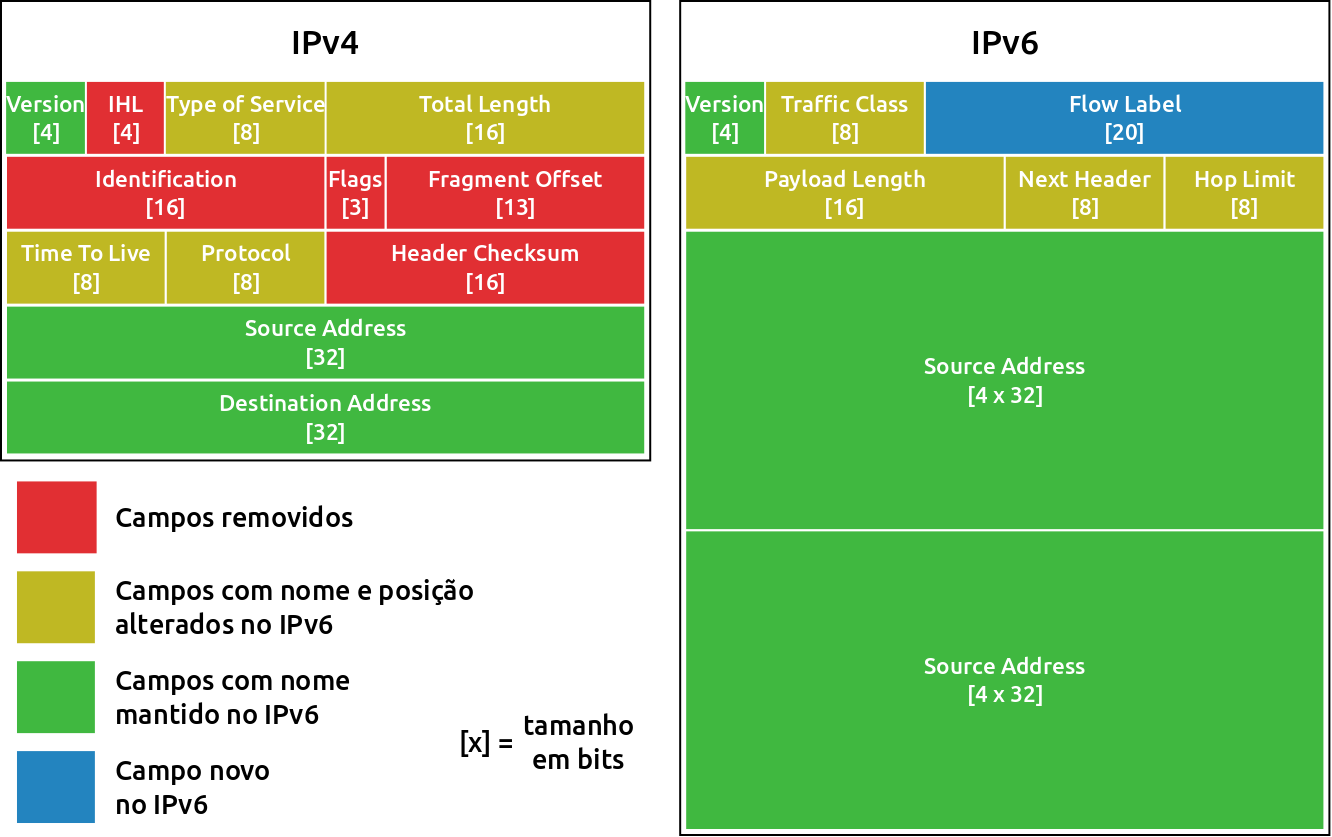
\includegraphics[width=\textwidth]{IPheaders.png}}
    \caption{formatos dos datagramas dos protocolos IPv4 e IPv6. Ambos possuem largura de 32 bits.}
    \label{fig:headers}
\end{figure}

Os campos do cabeçalho do IPv6 são:

\begin{description}
    \item[Version:] traz a versão do protocolo utilizado (no caso do IPv6, o valor 6).
        Porém, o simples envio do valor 4 não implica na utilização do IPv4, não
        possuindo compatibilidade anterior;

    \item[Traffic Class:] campo de 8 bits que possui a mesma finalidade do campo
        \emph{Type of Service} no IPv4, que especifica que o datagrama possui dados que
        requerem tráfego com baixo atraso, alta vazão ou confiabilidade;

    \item[Flow Label:] campo de 20 bits usado na classificação de fluxo de datagramas;

    \item[Payload Length:] campo de 16 bits que representa um inteiro positivo para o
        tamanho do conjunto de dados anexado após o cabeçalho;

    \item[Next Header:] identifica o protocolo usado para entregar os dados (\gls{tcp}
        ou \gls*{udp}). É usado da mesma forma que no IPv4;

    \item[Hop Limit:] quantidade máxima de roteadores pelos quais o datagrama poderá
        passar, sendo decrescido de 1 cada vez que passa por algum. Quando chega a 0, o
        datagrama é descartado; e

    \item[Source Address e Destination Address:] endereços IPv6 de origem e de destino
        do datagrama, em alguma das várias representações possíveis definidas no RFC4291
        \cite{site:rfcipv6add}.
\end{description}

Duas ausências significativas foram as dos campos que definem a fragmentação dos
datagramas e do \gls{checksum} do cabeçalho. No primeiro, a funcionalidade foi movida
dos roteadores, a fim de reduzir o trabalho deles e melhorar a velocidade do
encaminhamento IP pela rede, tornando os sistemas finais responsáveis pela escolha do
tamanho dos datagramas. Já no \gls*{checksum}, os protocolos das camadas de transporte
(\gls*{tcp} e \gls*{udp}) e de enlace (Ethernet) já realizam a verificação de erros por
soma. Por isso, a redundância de trabalho foi retirada, eliminando a necessidade de
recalcular essa soma a cada roteador e, assim, melhorando a velocidade de processamento
de pacotes IP.

Apesar de não ser retro-compatível com o IPv4, o IPv6 consegue ser transmitido utilizando
\textbf{tunelamento automático} por \textbf{mecanismos de transição}, que proporciona
uma camada transparente para que pacotes IPv6 transitem em uma rede IPv4. Entre esses
mecanismos estão o 6to4, 6in4 e Teredo.

%!TEX root = ../../tcc.tex

\subsection*{Uso do IPv6}

O IPv6 tem duas datas marcantes: o Dia Mundial e o Dia do Lançamento Mundial do IPv6.
No Dia Mundial do IPv6, ou \emph{World IPv6 Day}, organizado pelo
\emph{Internet Society} (ISOC) \cite{site:isoc-ipv6day}, ocorreu no dia 8 de junho de
2011 UTC e contou com a participação de grandes empresas estrangeiras (Facebook,
Google, Yahoo!, Akamai, Lamelight Networks, etc) e brasileiras (Terra, Campus Party,
IG), num teste de 24 horas de oferecimento de conexão e conteúdo utilizando o protocolo
IPv6. O evento foi considerado um sucesso pela ISOC.

Já o Dia de Lançamento Mundial do IPv6, no dia 6 de junho de 2012, foi um evento
semelhante ao Dia Mundial, com o mesmo objetivo e com mais participantes, porém mantendo
o IPv6 habilitado após o evento \cite{site:isoc-ipv6launch}. Desde então, empresas do
mundo todo têm corrido contra o relógio para que o oferecimento de conexões de Internet
não seja estagnado pela falta de endereços.

O IPv6 precisa ser suportado pelas pontas das redes (aplicações em clientes e
servidores) e pelas rotas entre eles (provedores de acesso, empresas de
telecomunicações). Enquanto o primeiro é simples, pois bastam configurações de
conectores dos respectivos sistemas operacionais, servidores de aplicação e roteadores
internos que suportem o IPv6, o caminhos entre ambos é mais complicado. Para as empresas
provedoras de acesso, envolvem custos de troca de equipamentos da infraestrutura de
rede, além do treinamento da mão de obra. Por conta disso, a transição para o novo
protocolo ainda é complexa e lenta.

O contexto brasileiro do IPv6 a situação está devagar. Segundo o SindiTelebrasil em
novembro de 2013 \cite{site:ipv6brasil}, as operadoras brasileiras ainda estavam
adquirindo equipamentos. O cenário era considerado preocupante, e devido ao atraso da
migração tecnológica, medidas paliativas estão sendo tomadas.

Uma delas é o compartilhamento de endereços IPv4 por usuários, com restrição de portas,
que pode afetar a experiência de uso de alguns tipos de aplicações. Esse
compartilhamento é feito usando-se dois \glspl*{nat}, usando o modelo de \gls*{nat}444.

\begin{figure}[H]
    \centering
    \fbox{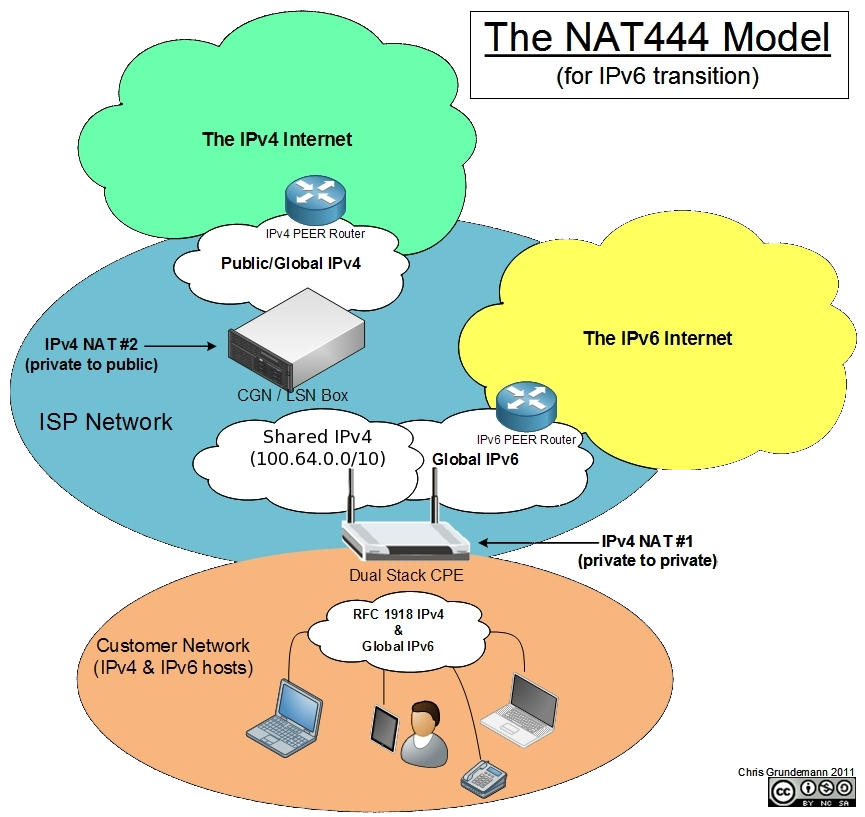
\includegraphics[width=\textwidth]{nat444.png}}
    \caption{Esquema de uso do NAT444. Fonte:\cite{site:nat444}}
    \label{fig:nat444}
\end{figure}

No \gls*{nat}444 \cite{site:nat444}, dois \glspl*{nat} são usados, e é possível perceber que:

\begin{itemize}
    \item \gls*{nat}444 de IPv4 funcionando em pilha dupla (\emph{dual stacked}; para
        ambos os protocolos) com IPv6 global (público); e

    \item \gls*{nat}444 adiciona uma segunda camada de \gls*{nat}, ou seja, uma segunda
        área de endereçamento ``interno'' (privada).
\end{itemize}

Ao adicionar a segunda camada, vários usuários podem ter um mesmo endereço, ou seja, o
\gls*{isp} deverá tomar medidas como registrar os acessos com as respectivas portas de
entrada e saída, por questões legais. Outro fato é que deve-se aceitar que o segundo
\gls*{nat} não será configurável por UPnP, por \gls*{nat}-PMP ou outros protocolos de
travessia de \gls*{nat}. Um \gls*{isp} não permitirá que ocorra essa configuração, pois
existirá o risco de um usuário afetar serviços de outros. Por esse motivo, pode-se
prever aplicações que podem ser afetadas com problemas de desempenho ou mesmo
incapacidade de execução \cite{site:rfcnat444}:

\begin{itemize}
    \item grandes downloads por FTP
    \item \emph{seeding} em Limewire e BitTorrent
    \item jogos online (Xbox, Playstation, etc)
    \item \emph{streaming} de vídeo (Hulu, Netflix, etc)
    \item acesso remoto de webcam
    \item tunelamento para IPv6 (6to4, Teredo, etc)
    \item VPN e criptografia (IPSec, SSL)
    \item VoIP
\end{itemize}

%!TEX root = ../../tcc.tex

\section{Conexão com a Internet}

Programas que se conectam à redes ou à Internet são comuns atualmente. Para isso, a
linguagem C permite escrever programas que criam conexões de Internet via \glspl{socket}
\cite{site:beej}.

Através de um \gls*{socket}, a aplicação consegue enviar mensagens para a camada de
transporte, que as transforma em segmentos e as repassa para as camadas inferiores, que
transmitem os dados.

Quando o protocolo \gls{tcp} for usado, os passos para se criar uma conexão serão:

\begin{enumerate}
    \item configuração do \gls*{socket} em uma variável \textbf{sadd} do tipo
        \sverb|struct sockaddr_in| (para IPv4) ou \sverb|struct sockaddr_in6| (para
        IPv6), que conterá informações do computador de destino da conexão.

        Enquanto isso, ocorre a criação de um \gls*{socket} usando a função
        \sverb|socket()|. Essa função, passando o parâmetro \bverb|SOCK_STREAM|, pede
        para o SO (sistema operacional) a criação de um descritor de arquivo especial
        para \gls*{socket} \gls*{tcp}, que será usado para o fluxo de dados da conexão;

    \item ligação do \gls*{socket} à variável \textbf{sadd} usando a função
        \sverb|bind()|, que serve para registrar no SO que ele deve manipular os dados
        que chegam na porta indicada em \textbf{sadd}, usando o \gls*{socket} indicado;

    \item aguardar conexões no \gls*{socket} usando a função \sverb|listen()|; e

    \item receber dados pelo \gls*{socket} usando a função \sverb|accept()|.
\end{enumerate}

\cfile[label="./libtransmission/net.c:317"]{./Codes/chap4/018-net-tcp.c}

\cfile[label="./libtransmission/net.c:417"]{./Codes/chap4/019-net-tcp2.c}

Já quando o protocolo \gls{udp} for usado, os passos para se criar uma conexão são
exatamente os mesmos que os do protocolo \gls*{tcp}, exceto pelo parâmetro
\bverb|SOCK_DGRAM| na função \sverb|socket()|.

\cfile[label="./libtransmission/tr-udp.c:190"]{./Codes/chap4/020-net-udp.c}

As funções \sverb|send()| e \sverb|recv()|, que enviam e recebem dados, respectivamente,
possuem as suas versões mais complexas \sverb|sendto()| e \sverb|recvfrom()|, recebendo
outro \gls*{socket} como parâmetro de entrada.

%!TEX root = ../../tcc.tex

\section{Retomada de downloads}

No Transmission e em algums outros softwares que realizam downloads, existe a função de
se pausar a transferência do arquivo para que seja retomado em outro momento. Nesta
seção, mostrarei qual a idéiapor trás desse mecanismo e a forma como foi implementado no
Transmission.

%!TEX root = ../../tcc.tex

\section{Threads}

Dentro de um contexto de programas que utilizam a Internet e funcionalidades que chegam
próximas ao tempo real, processamentos pesados devem ser tratados com cautela a fim de
se manter a instantaneidade do processo. Aqui explicarei como o Transmission usa o
conceito de \emph{threads} para paralelizar esses processamentos e, com isso, conseguir
utilizar as informações de rápida mudança antes que seja necessário obtê-las novamente.

%!TEX root = ../../tcc.tex

\section{Engenharia de Software}

O Transmission é um programa extenso e complexo, desenvolvido por vários programadores
que estão espalhados pelo globo. Nesta seção, abordarei alguns pontos utilizados pelos
desenvolvedores na manutenção do código aberto de qualidade e em funcionamento.

\afterpage{\clearpage}